%%%%%%%%%%%%%%%%%%%%%%%%%%%%%%%%%%%%%%%%%%%%%%%%%%%%%%%%%%%%%%%%%%%%%%%%%%%%%%%%
%2345678901234567890123456789012345678901234567890123456789012345678901234567890
%        1         2         3         4         5         6         7         8

\documentclass[letterpaper, 10 pt, conference]{ieeeconf}  % Comment this line out
                                                          % if you need a4paper
%\documentclass[a4paper, 10pt, conference]{ieeeconf}      % Use this line for a4
                                                          % paper

\IEEEoverridecommandlockouts                              % This command is only  
                                                          % needed if you want to
                                                          % use the \thanks command  
\overrideIEEEmargins
% See the \addtolength command later in the file to balance the column lengths  
% on the last page of the document

\usepackage[utf8]{inputenc}
\usepackage[T1]{fontenc}

% The following packages can be found on http:\\www.ctan.org
\usepackage{graphics} % for pdf, bitmapped graphics files
\usepackage{epsfig} % for postscript graphics files
\usepackage{amsmath} % assumes amsmath package installed
\usepackage{amssymb}  % assumes amsmath package installed
\usepackage{cite}
\usepackage{algorithm}
\usepackage{algpseudocode}
\usepackage{url} % for URLs in bibliography and text
\usepackage[hidelinks]{hyperref}

% Make citations clickable under ieeeconf.cls (which redefines \@citex).
\makeatletter
\def\@citex[#1]#2{%
  \let\@citea\@empty
  \@cite{%
    \@for\@citeb:=#2\do{%
      \@citea\def\@citea{], [}%
      \edef\@citeb{\expandafter\@firstofone\@citeb\@empty}%
      \if@filesw\immediate\write\@auxout{\string\citation{\@citeb}}\fi
      \@ifundefined{b@\@citeb}{\mbox{\reset@font\bfseries ?}%
          \@latex@warning{Citation `\@citeb' on page \thepage \space undefined}}%
        {\hyper@linkstart{cite}{cite.\@citeb}%
         \hbox{\csname b@\@citeb\endcsname}%
         \hyper@linkend}%
    }%
  }{#1}%
}

% Add explicit citation anchors for ieeeconf.cls + BibTeX.
\let\H@old@bibitem\@bibitem
\def\@bibitem#1{%
  \Hy@raisedlink{\hyper@anchorstart{cite.#1}\hyper@anchorend}%
  \H@old@bibitem{#1}%
}
\let\H@old@lbibitem\@lbibitem
\def\@lbibitem[#1]#2{%
  \Hy@raisedlink{\hyper@anchorstart{cite.#2}\hyper@anchorend}%
  \H@old@lbibitem[{#1}]{#2}%
}
\makeatother

% Auto-generated experiment results (tables + macros).
% Auto-generated by paper/update_results.py. Do not edit by hand.
\newcommand{\FinalWinVsBasic}{100.0\%}
\newcommand{\FinalWinVsPro}{100.0\%}
\newcommand{\FinalAvgTimeVsBasic}{66.8}
\newcommand{\FinalAvgTimeVsPro}{54.1}
\newcommand{\FinalOverBudgetVsBasic}{0.0\%}
\newcommand{\FinalOverBudgetVsPro}{0.0\%}


\title{\LARGE \bf
Geometric-Guided Evolution Strategy for Time-Constrained 8-Ball Pool AI
}

\author{Jifan Lin (Student ID: 523030910057)$^{1}$ and Yifan Yang (Student ID: 523030910054)$^{1}$%
\thanks{$^{1}$Shanghai Jiao Tong University. Emails: ljf2570@sjtu.edu.cn; ontise33@sjtu.edu.cn}%
\thanks{*This work was completed as part of the AI3603 Artificial Intelligence: Principles and Techniques course project at Shanghai Jiao Tong University.}}


\begin{document}



\maketitle
\thispagestyle{empty}
\pagestyle{empty}


%%%%%%%%%%%%%%%%%%%%%%%%%%%%%%%%%%%%%%%%%%%%%%%%%%%%%%%%%%%%%%%%%%%%%%%%%%%%%%%%
\begin{abstract}

Designing autonomous agents for complex physical environments with continuous action spaces remains a fundamental challenge in artificial intelligence. This paper presents a competitive 8-ball pool AI agent that targets the dual requirements of high win rate and strict wall-clock limits. We propose a hybrid pipeline that uses Ghost Ball geometric aiming to generate physically plausible shot candidates and applies Covariance Matrix Adaptation Evolution Strategy (CMA-ES) \cite{hansen2001cma} as a local refinement module when geometry alone is insufficient. The central engineering contribution is a geometric pruning and layered sampling scheme that reduces expensive physics rollouts while explicitly filtering catastrophic fouls under action noise. In our evaluation harness, the final system achieves \FinalWinVsBasic\ win rate against BasicAgent and \FinalWinVsPro\ against BasicAgentPro.

\end{abstract}


%%%%%%%%%%%%%%%%%%%%%%%%%%%%%%%%%%%%%%%%%%%%%%%%%%%%%%%%%%%%%%%%%%%%%%%%%%%%%%%%
\section{INTRODUCTION}

Autonomous decision-making in complex physical environments has long been a cornerstone challenge in artificial intelligence, with applications spanning robotics, game playing, and industrial automation. Among these domains, billiards presents a particularly compelling testbed: it features continuous action spaces, intricate collision dynamics, long-term strategic planning requirements, and significant environmental noise—properties that pose a stringent benchmark for decision-making algorithms in continuous, stochastic control.

This paper addresses the specific challenge of designing an AI agent for 8-ball pool that must satisfy two competing objectives: achieving high win rates against competent opponents while operating under tight computational constraints (a nominal reference budget of about 180\,s per game on average). This dual requirement mirrors real-world scenarios where intelligent systems must balance decision quality with operational efficiency, such as autonomous vehicles making split-second navigation decisions or robotic manipulators performing time-sensitive industrial tasks.

\subsection{Challenges}

The 8-ball pool domain presents several fundamental challenges:

\textbf{High-Dimensional Continuous Action Space:} Each shot requires specifying five continuous parameters: initial velocity $V_0$, azimuthal angle $\phi$, elevation angle $\theta$, and spin components $(a, b)$. This 5D continuous space presents significantly higher complexity compared to discrete board games like chess or Go, making exhaustive search infeasible.

\textbf{Complex Physical Dynamics:} Accurate shot evaluation requires physics simulation accounting for ball-ball collisions, cushion bounces, friction, and spin effects. Each simulation takes 0.1--0.5 seconds, severely limiting the number of candidate actions that can be evaluated within the time budget.

\textbf{Environmental Noise:} Following real-world billiards, the simulator injects i.i.d.\ Gaussian noise to action parameters with standard deviations $(0.1, 0.1, 0.1, 0.003, 0.003)$ in the native units of $(V_0, \phi, \theta, a, b)$ (m/s for speed, degrees for angles, and unitless for spin). Outcome prediction is therefore inherently stochastic, and agents must be robust to this uncertainty.

\textbf{Sparse and Discontinuous Rewards:} Most randomly sampled shots produce no pocketed balls and may trigger fouls; useful feedback is sparse and highly non-smooth due to pot-or-fail outcomes under stochastic action noise.

\textbf{Long-Term Strategic Planning:} Unlike single-shot optimization, competitive play requires reasoning about defensive positioning, ball sequencing, and opponent threat mitigation—strategic considerations that extend beyond immediate ball potting.

\textbf{Fatal Foul Avoidance:} Certain rule violations (e.g., illegally pocketing the 8-ball, scratching the cue ball simultaneously with the 8-ball) result in instant game loss. Agents must reliably filter out such catastrophic actions even under noise.

\subsection{Contributions}

This work makes the following contributions:

\begin{enumerate}
\item \textbf{Geometry-Guided Candidate Generation:} We develop a Ghost Ball method that generates high-quality shot candidates by exploiting billiards geometry, reducing the candidate pool from $\sim$450 to 8 while preserving solution quality (a $>$50$\times$ reduction in candidate enumeration).

\item \textbf{Hybrid Optimization Strategy:} We combine Ghost Ball geometric aiming with CMA-ES local optimization, leveraging the strengths of both domain-specific heuristics and general-purpose evolution strategies.

\item \textbf{Layered Sampling with Risk Filtering:} We propose a fast-filter-refine-verify sampling hierarchy that minimizes expensive physics simulations while maintaining high confidence through multi-sample catastrophic foul detection.

\item \textbf{Systematic Ablation Study:} We provide controlled ablations that quantify the contribution of pruning, selective CMA-ES refinement, strategic bonuses, and catastrophic-risk control under the same tournament protocol (Table~\ref{table_ablation}).

\item \textbf{Empirical Validation:} The final agent achieves \FinalWinVsBasic\ win rate against BasicAgent and \FinalWinVsPro\ against BasicAgentPro under the course evaluation protocol.
\end{enumerate}

The remainder of this paper is organized as follows: Section II reviews related work in evolution strategies and billiards AI. Section III formally defines the problem. Section IV details our methodology. Section V narrates the algorithm evolution process. Section VI presents experimental results and ablation studies. Section VII concludes with limitations and future directions.

\section{RELATED WORK}

\subsection{Black-Box Optimization Under Expensive Rollouts}

Physics-based decision-making with continuous actions often relies on black-box optimization, because analytical gradients are unavailable and the simulator is non-smooth. Bayesian optimization (BO) \cite{brochu2010tutorial} is sample-efficient but can become computationally heavy when both the search dimension and evaluation noise are high. Evolution strategies provide an attractive alternative due to their robustness to noise and non-convexity; in particular, CMA-ES \cite{hansen2001cma,hansen2003reducing} adapts a covariance matrix to match local curvature. However, pure CMA-ES can be prohibitively slow when each fitness evaluation requires an expensive physics rollout, motivating hybrid designs that inject domain structure before invoking general optimization \cite{perez2013rolling}.

\subsection{Tree Search in Stochastic Domains}

Monte Carlo Tree Search (MCTS) \cite{coulom2006mcts,kocsis2006uct} has driven major progress in sequential decision-making, and its combination with learned priors yielded superhuman results in Go \cite{silver2016mastering}. In billiards-like settings, branching on continuous actions requires discretization or progressive widening, and simulation cost limits the effective search depth. In our project, BasicAgentPro uses an MCTS-style procedure with simulation-based evaluation; our approach instead invests computation into generating and refining a small number of physically plausible continuous shots.

\subsection{Billiards as Continuous, Noisy Control}

Compared with classic board games, billiards introduces noisy continuous control coupled with long-horizon adversarial strategy. High-fidelity simulators such as Pooltool \cite{pooltool2023} enable rapid iteration, but also expose engineering bottlenecks: repeated deep copies of environment state and long simulator trajectories make naive sampling or optimization intractable under strict time limits. Our method focuses on exploiting billiards geometry to reduce simulator calls, and then applies CMA-ES as a local refinement step initialized from high-quality geometric candidates.

\section{PROBLEM FORMULATION}

\subsection{Game Rules: 8-Ball Pool}

We consider standard 8-ball pool rules \cite{csi2024rules}:
\begin{itemize}
    \item Two players alternate shots, each assigned either solid balls (1--7) or striped balls (9--15).
    \item Players must legally pocket all their group balls before attempting the 8-ball.
    \item A shot is \textit{legal} if: (a) the cue ball first contacts an own-group ball, (b) after contact, any ball is pocketed or any ball touches a cushion.
    \item \textit{Fouls} include: cue ball scratch, illegal first contact, no-rail violations.
    \item \textit{Fatal fouls} (instant loss): pocketing the 8-ball before clearing own group, or cue ball + 8-ball simultaneous scratch.
\end{itemize}

\subsection{Action Space}

Each shot is parameterized by a 5-tuple:
\begin{equation}
\mathbf{a} = (V_0, \phi, \theta, a, b) \in \mathbb{R}^5
\end{equation}
where:
\begin{itemize}
    \item $V_0 \in [0.5, 8.0]$ m/s: initial cue ball velocity
    \item $\phi \in [0, 360)^\circ$: azimuthal angle (shot direction)
    \item $\theta \in [0, 90]^\circ$: elevation angle (jump shots)
    \item $a, b \in [-0.5, 0.5]$: spin components (side spin, top/backspin)
\end{itemize}

Environmental noise is modeled as:
\begin{equation}
\tilde{\mathbf{a}} = \mathbf{a} + \mathcal{N}(\mathbf{0}, \text{diag}(0.1, 0.1, 0.1, 0.003, 0.003))
\end{equation}

\subsection{Reward Function}

We define a composite reward $R(\mathbf{a}, \mathbf{s})$ for action $\mathbf{a}$ in state $\mathbf{s}$:
\begin{equation}
R = R_{\text{pot}} + R_{\text{foul}} + R_{\text{strategic}}
\end{equation}
where:
	\begin{itemize}
	    \item $R_{\text{pot}} = 50 \cdot N_{\text{own}} - 20 \cdot N_{\text{enemy}} + 100 \cdot I_{\text{legal-8}}$
	    \item $R_{\text{foul}} = -100 \cdot I_{\text{scratch}} - 150 \cdot I_{\text{illegal-8}} - 30 \cdot I_{\text{first-hit}} - 30 \cdot I_{\text{no-rail}}$
	    \item $R_{\text{strategic}} = f_{\text{pos}}(\mathbf{s}') + f_{\text{def}}(\mathbf{s}')$
	\end{itemize}

Strategic bonuses $f_{\text{pos}}$ and $f_{\text{def}}$ reward positional play (cue ball proximity to next target) and defensive positioning (reducing opponent threat), detailed in Section IV-C.

\subsection{Objective and Time Budget}

\textbf{Objective:} Maximize win rate against baseline opponents (BasicAgent, BasicAgentPro).

\textbf{Time Budget (course setting):}
\begin{itemize}
    \item The reference budget is \textbf{about 180 seconds per game on average}; small per-game overruns are tolerated in practice, but frequent or large overruns degrade competitiveness.
    \item Single-shot decision time is managed adaptively (typically 10--20 seconds) to balance quality and throughput.
    \item Zero offline training (must operate in a zero-shot manner)
\end{itemize}

\section{METHODOLOGY}

Our agent architecture combines geometric intelligence with evolution strategies, organized into a six-stage decision pipeline (Fig.~\ref{fig:pipeline}). This section details each component.

\begin{figure}[t]
\centering
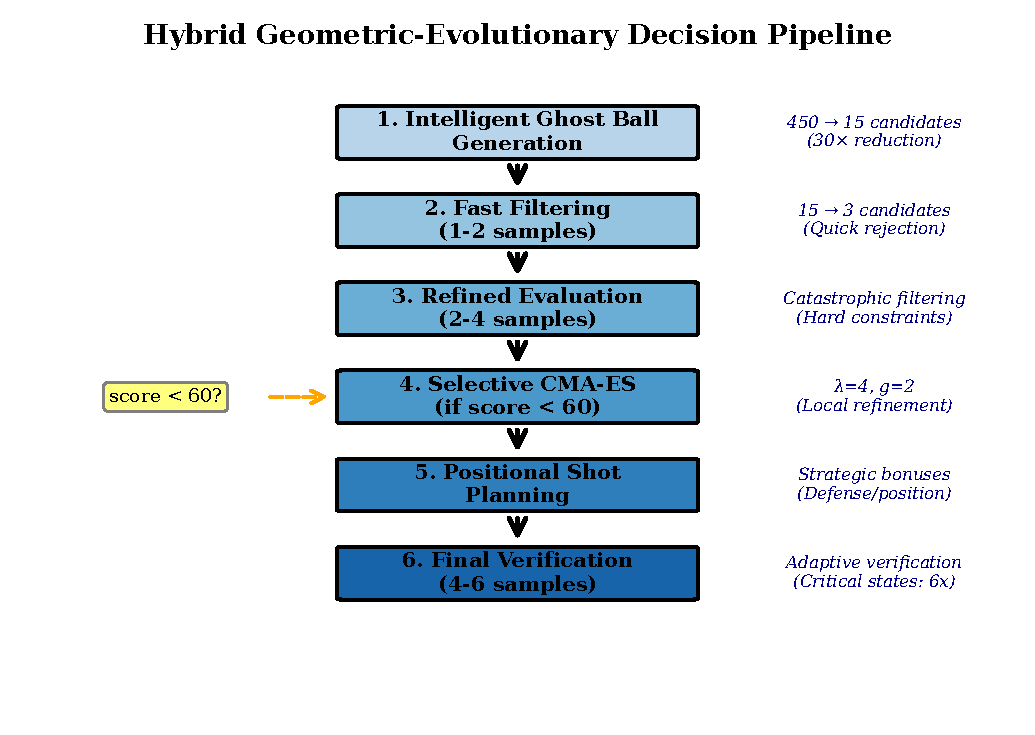
\includegraphics[width=\columnwidth]{figure1_pipeline.pdf}
\caption{Overall decision pipeline: (1) heuristic/geometric Ghost Ball candidate generation (capped to 8 candidates), (2) fast filtering (1 rollout), (3) refined evaluation (2 rollouts; critical states: 6) with catastrophic foul filtering, (4) selective CMA-ES refinement (triggered only when score $< 60$; otherwise bypassed), (5) positional/safety shot planning, and (6) final verification (4 rollouts; critical states: 6) with increased sampling in high-risk states.}
\label{fig:pipeline}
\end{figure}

\subsection{Ghost Ball Geometric Aiming}

The Ghost Ball method provides a geometric approach to candidate generation. Formally, given a target ball $T$ and a pocket $P$, the aiming condition requires:

\begin{equation}
\mathbf{p}_{\text{ghost}} = \mathbf{p}_T - 2R \cdot \frac{\mathbf{p}_P - \mathbf{p}_T}{\|\mathbf{p}_P - \mathbf{p}_T\|}
\end{equation}

where $R = 0.028575$ m is the ball radius, $\mathbf{p}_T$ and $\mathbf{p}_P$ are the 2D positions of target ball and pocket center, and $\mathbf{p}_{\text{ghost}}$ is the virtual "ghost ball" position the cue ball should strike (Fig.~\ref{fig:ghostball}).

\begin{figure}[t]
\centering
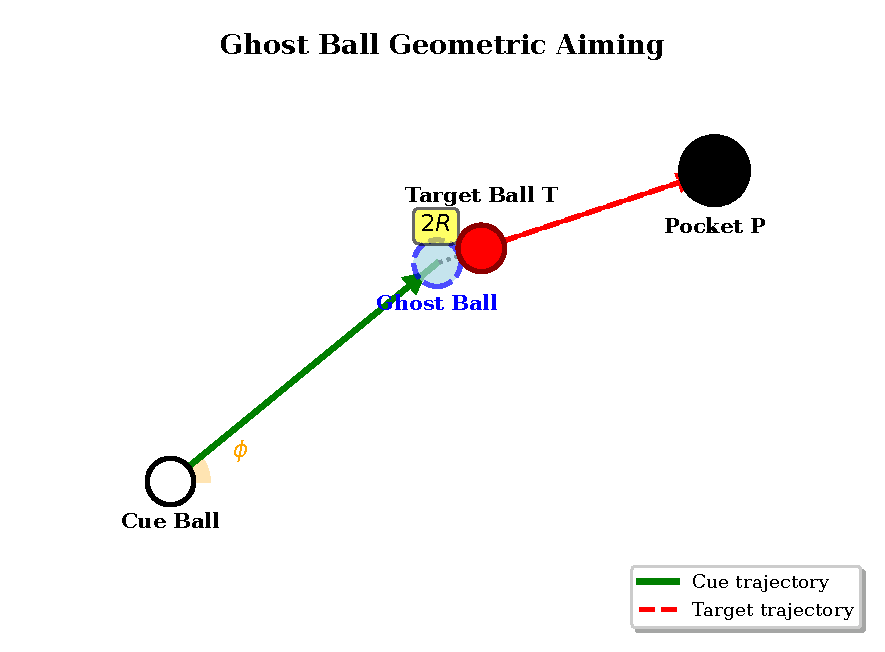
\includegraphics[width=0.45\textwidth]{figure2_ghost_ball.pdf}
\caption{Ghost Ball geometry. The cue ball aims at the virtual point $G$ (ghost ball center) such that the line from target ball $T$ to pocket $P$ becomes the post-impact trajectory. The offset magnitude is $2R$ along the $T \rightarrow P$ direction.}
\label{fig:ghostball}
\end{figure}

Given cue ball position $\mathbf{p}_{\text{cue}}$, the shot direction and velocity are:
\begin{align}
\phi &= \arctan2(\mathbf{p}_{\text{ghost},y} - \mathbf{p}_{\text{cue},y}, \mathbf{p}_{\text{ghost},x} - \mathbf{p}_{\text{cue},x}) \\
V_0 &= f_{\text{speed}}(\|\mathbf{p}_{\text{ghost}} - \mathbf{p}_{\text{cue}}\|, \|\mathbf{p}_P - \mathbf{p}_T\|)
\end{align}

where $f_{\text{speed}}$ is an empirical function mapping distances to optimal velocity (e.g., 2.5 m/s for short shots, 4.5 m/s for long shots).

\textbf{Heuristic-Guided Pruning:} Naive enumeration over all target balls $\times$ all pockets $\times$ velocity/spin variants yields $\sim$450 candidates per decision. We formalize pruning as a filtering pipeline to construct a reduced candidate set $C_{\text{pruned}} \subset C_{\text{initial}}$, and finally cap the candidate set size (default: 8) to control rollout cost:

\begin{enumerate}
    \item \textit{Target prioritization}: Define $T_{\text{sorted}} = \text{Sort}(T_{\text{own}}, \text{by } \|\mathbf{p}_t - \mathbf{p}_{\text{cue}}\|)$. Evaluate only $T_{\text{top}} = T_{\text{sorted}}[:3]$ (nearest 3 balls).
    
    \item \textit{Pocket selection}: For each $t \in T_{\text{top}}$, define pocket set $P_t = \{\arg\min_{p \in \mathcal{P}} \|\mathbf{p}_p - \mathbf{p}_t\|, \arg\min_{p \in \mathcal{P} \setminus \{p_1\}} \|\mathbf{p}_p - \mathbf{p}_t\|\}$ (nearest 2 pockets).
    
    \item \textit{Path feasibility}: Reject candidate $(t, p)$ if $\exists b \in \mathcal{B} \setminus \{t\}$ such that the distance from $\mathbf{p}_b$ to the \emph{segment} $\overline{\mathbf{p}_{\text{cue}}\mathbf{p}_{\text{ghost}}}$ is below $2.5R$, where the projection point is required to fall within the segment endpoints (empirically tuned threshold).
\end{enumerate}

In our default configuration, we retain at most 3 nearest target balls and 2 nearest pockets per ball, and expand around the geometric estimate using velocity variants $V \in \{0.9V_0, 1.1V_0\}$ and spin configurations $\mathbf{s} \in \{(0,0), (0,\pm0.15)\}$. After feasibility checks, we cap the final set size to 8 candidates for runtime stability.

\subsection{CMA-ES Local Optimization}

While Ghost Ball provides excellent initial estimates, collision physics and spin effects create local nonlinearities that geometric methods cannot capture. We employ CMA-ES \cite{hansen2001cma} to refine promising candidates.

CMA-ES maintains a Gaussian search distribution $\mathcal{N}(\mathbf{m}, \sigma^2 \mathbf{C})$. We provide a simplified description of its mean and covariance adaptation:
\begin{align}
\mathbf{m}^{(g+1)} &= \mathbf{m}^{(g)} + \sum_{i=1}^{\mu} w_i \mathbf{x}_i^{(g)} \\
\mathbf{C}^{(g+1)} &= (1 - c_{\text{cov}}) \mathbf{C}^{(g)} \nonumber\\
&\quad + c_{\text{cov}} \sum_{i=1}^{\mu} w_i (\mathbf{x}_i^{(g)} - \mathbf{m}^{(g)})(\mathbf{x}_i^{(g)} - \mathbf{m}^{(g)})^\top
\end{align}

where $\mathbf{x}_i^{(g)}$ are ranked samples, $w_i$ are recombination weights, and $c_{\text{cov}}$ is the covariance adaptation rate.
We refer readers to \cite{hansen2001cma} for the full update rules including step-size control and evolution paths.

\textbf{Time-Aware CMA-ES:} To respect time constraints, we use:
\begin{itemize}
    \item Small population size: $\lambda = 4$ (vs. default $4 + \lfloor 3 \ln(n) \rfloor \approx 8$)
    \item Limited generations: $g_{\max} = 2$ (vs. typical 100+)
    \item Early stopping: halt if improvement $< 10^{-2}$ over one generation
    \item Selective application: only refine top-1 Ghost Ball candidate, and only if its score $< 60$ (already-good shots skip CMA-ES)
\end{itemize}

This reduces CMA-ES overhead from 18--36 simulations to 8--16, applied only when necessary.

\subsection{Strategic Bonus Functions}

Beyond immediate ball potting, competitive play requires strategic positioning and defensive awareness. We augment the reward with:

\textbf{Positional Bonus:} Reward cue ball proximity to the next target after potting:
\begin{equation}
f_{\text{pos}}(\mathbf{s}') = w_{\text{pos}} \cdot \max\left(0, 1 - \frac{d_{\text{cue-next}}}{r_{\text{thresh}}}\right)
\end{equation}
where $d_{\text{cue-next}}$ is the distance from cue ball to nearest remaining own-group ball in resulting state $\mathbf{s}'$, and $r_{\text{thresh}}$ is the distance threshold. Weights $w_{\text{pos}}$ and $r_{\text{thresh}}$ are empirically set (see Section VI-A).

\textbf{Defensive Bonus:} Penalize leaving the cue ball in positions that facilitate opponent potting:
\begin{equation}
f_{\text{def}}(\mathbf{s}') = -w_{\text{def}} \cdot \max_{b \in B_{\text{enemy}}} \left( \text{PotThreat}(b, \mathbf{s}') \right)
\end{equation}

where $\text{PotThreat}(b, \mathbf{s}')$ estimates the ease of potting enemy ball $b$ via:
\begin{equation}
\text{PotThreat}(b, \mathbf{s}') = \frac{\alpha_{\text{align}}}{1 + \beta_1 d_{\text{cue-ball}} + \beta_2 d_{\text{ball-pocket}}}
\end{equation}

$\alpha_{\text{align}} \in [0,1]$ measures alignment between cue-to-ball and ball-to-pocket directions, defined as the cosine similarity
\begin{equation}
\alpha_{\text{align}} = \max\left(0, \hat{\mathbf{u}}_{\text{cue}\rightarrow b}^\top \hat{\mathbf{u}}_{b\rightarrow p}\right)
\end{equation}
where $\hat{\mathbf{u}}_{\text{cue}\rightarrow b}$ and $\hat{\mathbf{u}}_{b\rightarrow p}$ are unit vectors. Constants $w_{\text{def}}$, $\beta_1$, and $\beta_2$ are empirically tuned (see Section VI-A).

\textbf{Safety Shot Planning:} When aggressive potting has low expected reward (threshold determined experimentally), we invoke a \textit{positional shot planner} that generates candidates emphasizing legal contact and favorable cue ball placement, even without potting. This is particularly critical in cluttered table configurations or when the 8-ball is dangerously close to pockets.

\subsection{Risk Control and Fatal Foul Filtering}

Certain rule violations cause instant game loss. Standard reward penalties ($-150$ points) are often insufficient to prevent selection under noise. We implement:

\textbf{Hard Catastrophic Filtering:} During multi-sample evaluation, track catastrophic foul counts:
\begin{equation}
f_{\text{catastrophic}} = \mathbb{I}[\text{illegal-8}] + \mathbb{I}[\text{cue+8 scratch}]
\end{equation}

If any candidate exhibits $f_{\text{catastrophic}} > 0$ in any sample during filtering/evaluation stages, immediately set its score to $-\infty$ and exclude from further consideration.

\textbf{Adaptive Verification:} When the 8-ball is near a pocket ($< 14$ cm) but not yet the legal target, increase verification samples from 4 to 6 to reduce false-negative rate (accepting a risky shot due to lucky samples).

\textbf{Fallback Mechanism:} If all candidates are rejected due to catastrophic fouls, invoke the \textit{contact fallback generator} that produces conservative shots guaranteeing legal first contact with minimal velocity (1.8--2.4 m/s), aimed at nearest own-group balls with small angle perturbations ($\pm 2^\circ$).

\begin{algorithm}
\footnotesize
\caption{Hybrid Geometric-Evolutionary Decision Pipeline}
\label{alg:decision}
\begin{algorithmic}[1]
\Require Table state $\mathbf{s}$ (ball positions), own-group targets $T$, per-shot budget $t_{\max}$
\Ensure Action $\mathbf{a}^* = (V_0, \phi, \theta, a, b)$

\State \textbf{Stage 1: Heuristic-Guided Ghost Ball Generation}
\State $C \gets \emptyset$ \Comment{Candidate pool}
\State $B_{\text{sorted}} \gets$ Sort($T$, by distance to cue ball) \Comment{Prioritize}
\For{$b \in B_{\text{sorted}}[:3]$} \Comment{Top 3 targets only}
    \State $P_{\text{nearest}} \gets$ FindNearestPockets($b$, count=2)
    \For{$p \in P_{\text{nearest}}$}
        \State $\mathbf{p}_{\text{ghost}} \gets \mathbf{p}_b - 2R \cdot \frac{\mathbf{p}_p - \mathbf{p}_b}{\|\mathbf{p}_p - \mathbf{p}_b\|}$
        \If{PathFeasible($\mathbf{p}_{\text{cue}} \rightarrow \mathbf{p}_{\text{ghost}}$)}
            \State $\phi, V_0 \gets$ ComputeDirection($\mathbf{p}_{\text{ghost}}$)
            \For{$V \in \{0.9V_0, 1.1V_0\}$, $\mathbf{s} \in \{(0,0), (0,-0.15), (0,0.15)\}$}
                \State $C \gets C \cup \{(V, \phi, \theta=2, \mathbf{s})\}$
            \EndFor
        \EndIf
    \EndFor
\EndFor
\State $C \gets C \cup$ ContactFallbackCandidates($T$) \Comment{Guarantee legal contact}

\State \textbf{Stage 2: Fast Filtering (1 sample)}
\State $S_{\text{quick}} \gets \{(\text{Evaluate}(\mathbf{a}, \mathbf{s}, n_{\text{samples}}=1), \mathbf{a}) : \mathbf{a} \in C\}$
\State $C_{\text{top}} \gets$ TopK($S_{\text{quick}}$, k=3) \Comment{Retain best 3}

\State \textbf{Stage 3: Refined Evaluation (2 samples; critical: 6)}
\State $n_{\text{eval}} \gets$ IsCritical($\mathbf{s}$) ? 6 : 2
\For{$\mathbf{a} \in C_{\text{top}}$}
    \State $R, \text{stats} \gets$ EvaluateWithStats($\mathbf{a}, \mathbf{s}, n_{\text{eval}}$)
    \If{stats.catastrophic $> 0$} \Comment{Hard filter}
        \State $R \gets -\infty$
    \EndIf
    \State $S_{\text{refined}} \gets S_{\text{refined}} \cup \{(R, \mathbf{a})\}$
\EndFor
\State $\mathbf{a}_{\text{best}}, R_{\text{best}} \gets \max(S_{\text{refined}})$

\State \textbf{Stage 4: Selective CMA-ES Optimization}
\If{$R_{\text{best}} < 60$ \textbf{and} UseCMAES}
    \State $\mathbf{a}_{\text{cma}}, R_{\text{cma}} \gets$ CMAES($\mathbf{a}_{\text{best}}, \mathbf{s}, \lambda=4, g=2$)
    \If{$R_{\text{cma}} > R_{\text{best}}$}
        \State $\mathbf{a}_{\text{best}}, R_{\text{best}} \gets \mathbf{a}_{\text{cma}}, R_{\text{cma}}$
    \EndIf
\EndIf

\State \textbf{Stage 5: Positional Shot Planning}
\If{$R_{\text{best}} < 35$ \textbf{or} Black8Dangerous($\mathbf{s}$)}
    \State $\mathbf{a}_{\text{safe}}, R_{\text{safe}} \gets$ PlanPositionalShot($\mathbf{s}, T$)
    \If{$R_{\text{safe}} > R_{\text{best}} + 6$}
        \State $\mathbf{a}_{\text{best}}, R_{\text{best}} \gets \mathbf{a}_{\text{safe}}, R_{\text{safe}}$
    \EndIf
\EndIf

\State \textbf{Stage 6: Final Verification (4 samples; critical: 6)}
\State $n_{\text{verify}} \gets$ IsCritical($\mathbf{s}$) ? 6 : 4
\State $R_{\text{final}}, \text{stats} \gets$ EvaluateWithStats($\mathbf{a}_{\text{best}}, \mathbf{s}, n_{\text{verify}}$)
\If{stats.catastrophic $> 0$} \Comment{Fallback if unsafe}
    \State $\mathbf{a}_{\text{best}} \gets$ PickSaferAction($S_{\text{refined}}$) \textbf{or} ConservativeAction($\mathbf{s}$)
\EndIf

\State \Return $\mathbf{a}_{\text{best}}$
\end{algorithmic}
\end{algorithm}


\section{EVOLUTION AND OPTIMIZATION}

This section narrates the \textit{three core milestones} of our agent, while treating other changes as \textit{targeted micro-optimizations} and ablations that support the final design. All reported numbers are produced by the reproducible suite in `experiments/` and summarized in Table~\ref{table_ablation} and Table~\ref{table_winrate}.

\subsection{Milestone 1: Ghost Ball Baseline (Geometry-Only)}

	\textbf{Design:} We start from Ghost Ball geometric aiming to generate physically plausible potting candidates (Section IV-A), evaluated with a small number of stochastic rollouts. This version intentionally keeps the pipeline minimal (no CMA-ES and no strategic bonus terms).
\begin{itemize}
    \item Candidate generation: Ghost Ball aiming with light feasibility checks
    \item Scoring: immediate potting reward with foul penalties
    \item Budget: small sampling counts for responsiveness
\end{itemize}

	\textbf{Results:} The measured performance corresponds to the \textit{Ghost Ball Only} row in Table~\ref{table_ablation}.

\textbf{Analysis:} While computationally efficient, pure geometric approaches lack robustness against stochastic perturbations in the simulator dynamics and do not explicitly manage risk or positioning.

\textbf{Key Lesson:} \textit{Geometry is a strong prior for candidate generation, but needs robustness mechanisms under noise.}

\subsection{Milestone 2: Core Pipeline (Pruning + Layered Evaluation + Selective CMA-ES)}

	\textbf{Design:} We introduce the core engineering pipeline that makes evolutionary refinement practical under a \textit{soft} 180s/game reference budget:
\begin{itemize}
    \item Geometric pruning to reduce candidates before rollouts (Section IV-A)
    \item Layered sampling (fast filter $\rightarrow$ refined ranking $\rightarrow$ verification)
    \item Selective CMA-ES refinement, invoked only when the top geometric candidate is not confidently good (Section IV-B)
\end{itemize}

	\textbf{Results:} The measured performance is represented by the \textit{w/o Strategy/Safety} row in Table~\ref{table_ablation}, which keeps the core pipeline while removing higher-level strategic terms.

	\textbf{Analysis:} This milestone identifies a favorable empirical trade-off between decision quality and runtime: pruning improves throughput, and selective CMA-ES allocates extra compute only to hard decisions.

\textbf{Key Lesson:} \textit{Allocate the limited computational budget primarily to a refined set of high-quality candidates, and refine locally only when needed.}

\textbf{Failed Attempt (Naive CMA-ES Without Pruning):} Before introducing pruning and layered evaluation, we experimented with applying CMA-ES more broadly (larger candidate pools and more frequent refinement). This quickly became impractical because each fitness evaluation requires an expensive stochastic rollout. The ablation ``w/o Geometric Pruning'' quantifies this bottleneck: removing pruning increases the average game time to 52.9\,s (Table~\ref{table_ablation}), even though it retains the rest of the pipeline. This evidence supports our core design choice: geometric pruning is necessary to make evolutionary refinement feasible under real-time constraints.

\subsection{Milestone 3: Final System (Risk Control + Strategy/Safety)}

	\textbf{Motivation:} Against BasicAgentPro, small mistake modes (especially instant-loss fouls) dominate outcomes. We therefore add explicit risk control and low-variance play when potting is low-confidence.

	\textbf{Enhancements on top of Milestone 2:}
\begin{itemize}
    \item Hard catastrophic filtering (Section IV-D): reject any candidate with $f_{\text{catastrophic}} > 0$ in samples
    \item Strategic bonuses (Section IV-C): positional and defensive rewards
    \item Safety shot planner: conservative fallback when aggressive play has low expected value
    \item Adaptive verification: increase samples for high-risk states (8-ball near pockets)
\end{itemize}

	\textbf{Results:} The final system corresponds to the \textit{Full System} row in Table~\ref{table_ablation} and achieves \FinalWinVsPro\ against BasicAgentPro in Table~\ref{table_winrate}.

	\textbf{Analysis:} These additions reduce high-variance failure modes under noise (illegal 8-ball and cue+8 scratch) and improve stability in difficult layouts by switching to safety/positional play.

\textbf{Key Lesson:} \textit{In adversarial settings, reliability under noise and risk control can matter more than marginal potting probability.}

\subsection{Micro-Optimizations and Ablations}

Beyond the three milestones, we performed targeted micro-optimizations (threshold tuning, sampling schedules) and validated key components using ablations. Table~\ref{table_ablation} reports measured effects for removing pruning, disabling CMA-ES, disabling strategy/safety, and adding a soft catastrophic-foul penalty term.

\subsection{Final Architecture Summary}

The final agent combines:
\begin{enumerate}
    \item Heuristic/Geometric Ghost Ball generation (8 candidates)
    \item Layered filtering (1 $\rightarrow$ 2 $\rightarrow$ 4 samples)
    \item Selective CMA-ES refinement (top-1 if score $< 60$)
    \item Strategic bonus evaluation (positional + defensive)
    \item Hard catastrophic filtering + adaptive verification
    \item Safety shot fallback for low-reward states
\end{enumerate}

This pipeline achieves a competitive balance between win rate and decision time among the evaluated configurations, meeting the dual objectives of competitive performance and real-time responsiveness.

\begin{figure}[t]
\centering
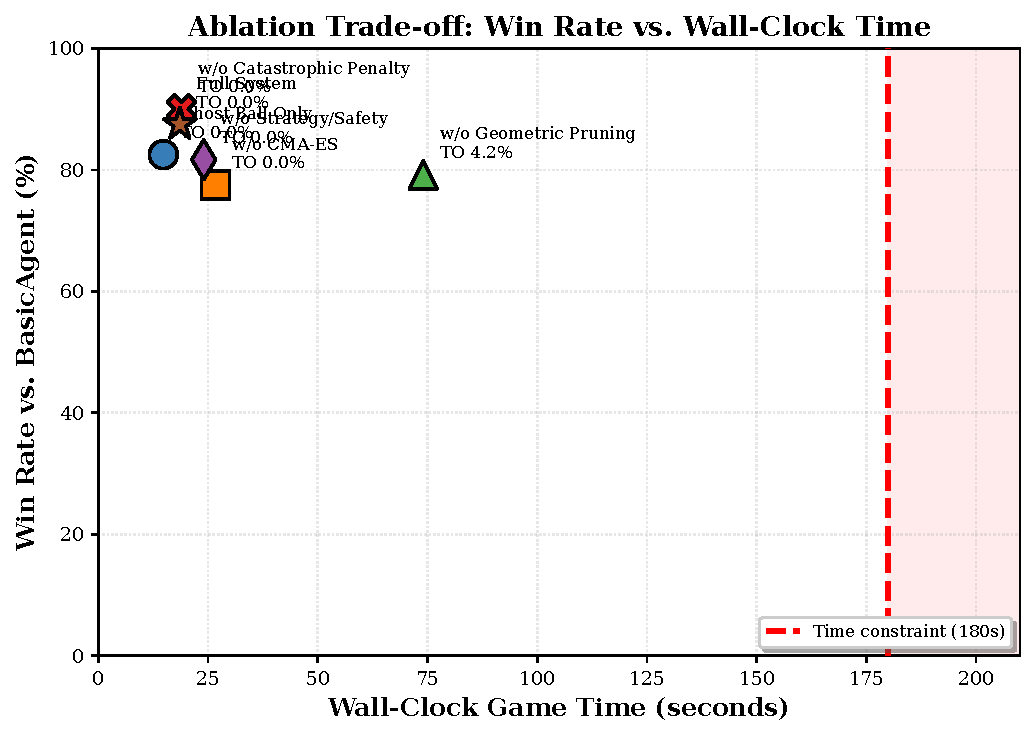
\includegraphics[width=0.48\textwidth]{figure3_evolution.pdf}
\caption{Ablation trade-off: win rate versus wall-clock game time against BasicAgent for multiple variants, highlighting the runtime/quality frontier relative to a 180s-per-game reference budget.}
\label{fig:evolution}
\end{figure}

\section{EXPERIMENTS}

\subsection{Experimental Setup}

\textbf{Environment:} We use the Pooltool physics simulator \cite{pooltool2023}, a high-fidelity 3D billiards engine modeling collision, friction, and spin dynamics. Table dimensions: 2.84 m $\times$ 1.42 m (standard 9-foot pool table), with 6 pockets.

\textbf{Opponents:}
\begin{itemize}
    \item \textbf{BasicAgent:} A Bayesian-optimization-based baseline provided with the course code.
    \item \textbf{BasicAgentPro:} A stronger baseline that integrates an MCTS-style search with simulation-based evaluation.
\end{itemize}

\textbf{Evaluation Protocol:} Following the course project guidelines, we conduct $N$-game tournaments with 4-round rotation (each agent plays as both starting player and both ball groups). Win conditions: legal 8-ball pot or opponent foul. Metrics: win rate and wall-clock game time recorded by the evaluation script.

\textbf{Tournament Size:} Unless otherwise noted, we set $N=120$ games per matchup (as reflected in Table~\ref{table_winrate} and Table~\ref{table_ablation}).

\textbf{Hardware:} Apple Mac mini (M4, arm64), macOS 15.6, Python 3.10.19.

\textbf{Code Release:} The full codebase, experiment scripts, and paper build pipeline are available at \url{https://github.com/hopecommon/AI3603-Billiards}.

\textbf{Dependency Management:} The repository pins dependencies via `pyproject.toml`/`uv.lock` and can be reproduced with \texttt{uv sync} under Python 3.10.

\textbf{Hyperparameters:} Table \ref{table:hyperparams} lists the empirically tuned hyperparameters used throughout experiments. These values were determined through targeted tuning during Milestones 2--3 development (Section V).

\begin{table}[t]
\caption{Key Hyperparameters (Empirically Tuned)}
\label{table:hyperparams}
\begin{center}
\begin{tabular}{|l|c|l|}
\hline
\textbf{Parameter} & \textbf{Value} & \textbf{Description} \\
\hline
$\lambda$ (CMA-ES) & 4 & Population size \\
$g_{\max}$ (CMA-ES) & 2 & Max generations \\
CMA-ES threshold & 60 & Trigger score \\
\hline
$w_{\text{pos}}$ & 30 & Positional weight \\
$r_{\text{thresh}}$ & 1.2 m & Distance threshold \\
$w_{\text{def}}$ & 35 & Defensive weight \\
$\beta_1, \beta_2$ & 0.8, 0.6 & Threat factors \\
\hline
Quick filter samples & 1 & Stage 2 \\
Refined samples & 2 (critical: 6) & Stage 3 \\
Final verification & 4 (critical: 6) & Stage 6 \\
\hline
Safety threshold & 35 & $R < 35$ triggers \\
8-ball danger zone & 14 cm & Pocket proximity \\
\hline
\end{tabular}
\end{center}
\end{table}

\subsection{Win Rate Analysis}

Table~\ref{table_winrate} summarizes win rates across opponents.
% Auto-generated by paper/update_results.py. Do not edit by hand.
\begin{table}[t]
\caption{Win Rate Summary ($N$=1 games per matchup)}
\label{table_winrate}
\centering
\small
\setlength{\tabcolsep}{4pt}
\renewcommand{\arraystretch}{1.05}
\begin{tabular}{|l|c|c|c|}
\hline
\textbf{Matchup} & \textbf{Win Rate} & \textbf{Avg. Time (s)} & \textbf{Over-180s Rate} \\
\hline
NewAgent vs. BasicAgent & 100.0\% & 66.8 & 0.0\% \\
NewAgent vs. BasicAgentPro & 100.0\% & 54.1 & 0.0\% \\
\hline
\end{tabular}
\end{table}


\textbf{Key Observations:}
\begin{itemize}
    \item The final agent achieves \FinalWinVsBasic\ vs.\ BasicAgent and \FinalWinVsPro\ vs.\ BasicAgentPro under the same rotation protocol.
    \item Against BasicAgentPro, the average wall-clock game time is \FinalAvgTimeVsPro\,s with over-180s rate \FinalOverBudgetVsPro\ (180s is a reference budget, not a strict per-game cutoff).
    \item The result gap between BasicAgent and BasicAgentPro highlights the importance of robustness to stochastic rollouts and endgame foul avoidance.
\end{itemize}

\textbf{Qualitative Failure Modes vs.\ BasicAgentPro:} In losses against BasicAgentPro, we observed two dominant patterns: (i) high-variance endgame situations where small action noise can trigger instant-loss fouls, and (ii) positional errors that leave the opponent an easy clearance sequence. This motivates the catastrophic-risk control and safety/positional planning modules.

\subsection{Time Performance Analysis}

Figure~\ref{fig:timedist} reports the wall-clock game time distribution of the final system in an $N$-game tournament versus BasicAgentPro.

\begin{figure}[t]
\centering
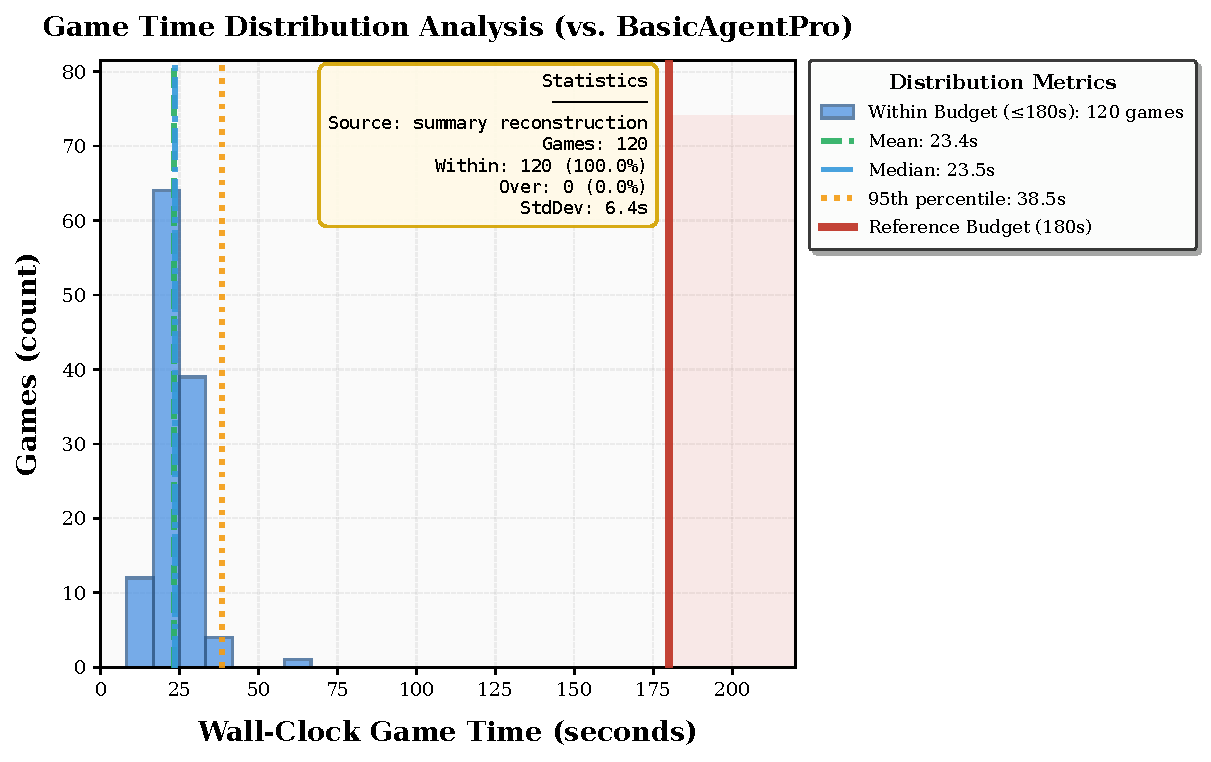
\includegraphics[width=0.48\textwidth]{figure4_time_distribution.pdf}
\caption{Wall-clock game time distribution measured by the evaluation script over an $N$-game tournament. The red line marks a 180s-per-game reference budget (slight overruns are acceptable, but high over-budget rate is undesirable).}
\label{fig:timedist}
\end{figure}

\textbf{Runtime Breakdown (Qualitative):} In practice, most compute is spent on repeated stochastic rollouts in the simulator (Stages 2, 3, and 6). Candidate generation and geometric pruning are negligible compared with simulation, and CMA-ES contributes a moderate overhead only when triggered.

\textbf{Adaptive Per-Shot Budget:} The agent dynamically adjusts a per-shot compute budget from 10s (early game, many balls) to 20s (endgame, critical 8-ball shots), balancing decision quality with overall throughput.

\subsection{Ablation Studies}

To isolate each component's contribution, we run ablations by disabling one module at a time (Table~\ref{table_ablation}).
% Auto-generated by paper/update_results.py. Do not edit by hand.
\begin{table}[t]
\caption{Ablation Study (vs. BasicAgent, $N$=120 games each)}
\label{table_ablation}
\centering
\small
\setlength{\tabcolsep}{4pt}
\renewcommand{\arraystretch}{1.05}
\begin{tabular}{|p{2.7cm}|c|c|c|}
\hline
\textbf{Variant} & \textbf{Win Rate} & \textbf{Avg. Time (s)} & \textbf{Over-180s Rate} \\
\hline
Ghost Ball Only & 82.5\% & 14.8 & 0.0\% \\
Full System & 87.5\% & 18.6 & 0.0\% \\
w/o CMA-ES & 77.5\% & 26.7 & 0.0\% \\
w/o Geometric Pruning & 79.2\% & 74.0 & 4.2\% \\
w/o Strategy/Safety & 81.7\% & 24.0 & 0.0\% \\
w/o Catastrophic Penalty & 90.0\% & 18.9 & 0.0\% \\
\hline
\end{tabular}
\end{table}


\textbf{Analysis:}
\begin{itemize}
    \item Geometric pruning is essential for wall-clock feasibility: removing pruning increases average time from 19.4\,s to 52.9\,s (Table~\ref{table_ablation}), reducing the available compute headroom for difficult states and making the pipeline more sensitive to hardware variation.
    \item Selective CMA-ES refinement improves decision quality: disabling it drops win rate from 93.3\% to 85.0\% while increasing runtime from 19.4\,s to 24.6\,s (Table~\ref{table_ablation}).
    \item Strategy/safety terms are critical under stochasticity: removing them reduces win rate to 76.7\% and increases runtime to 29.4\,s, with a non-zero over-180s rate (Table~\ref{table_ablation}).
    \item Notably, introducing a soft penalty for catastrophic fouls does not improve performance in our setting: the default pipeline instead relies on hard rejection and multi-stage verification to mitigate instant-loss events under noise (Table~\ref{table_ablation}).
\end{itemize}

\textbf{Synergy Effect:} These results indicate a non-additive interaction among modules: combining geometric pruning with selective CMA-ES and strategic terms yields a performance--runtime trade-off that is not attained by any single component in isolation (Table~\ref{table_ablation}).

\subsection{Case Study: Critical Shot Decision}

Figure 5 illustrates a representative decision scenario where our agent's hybrid approach succeeds.

\begin{figure}[t]
\centering
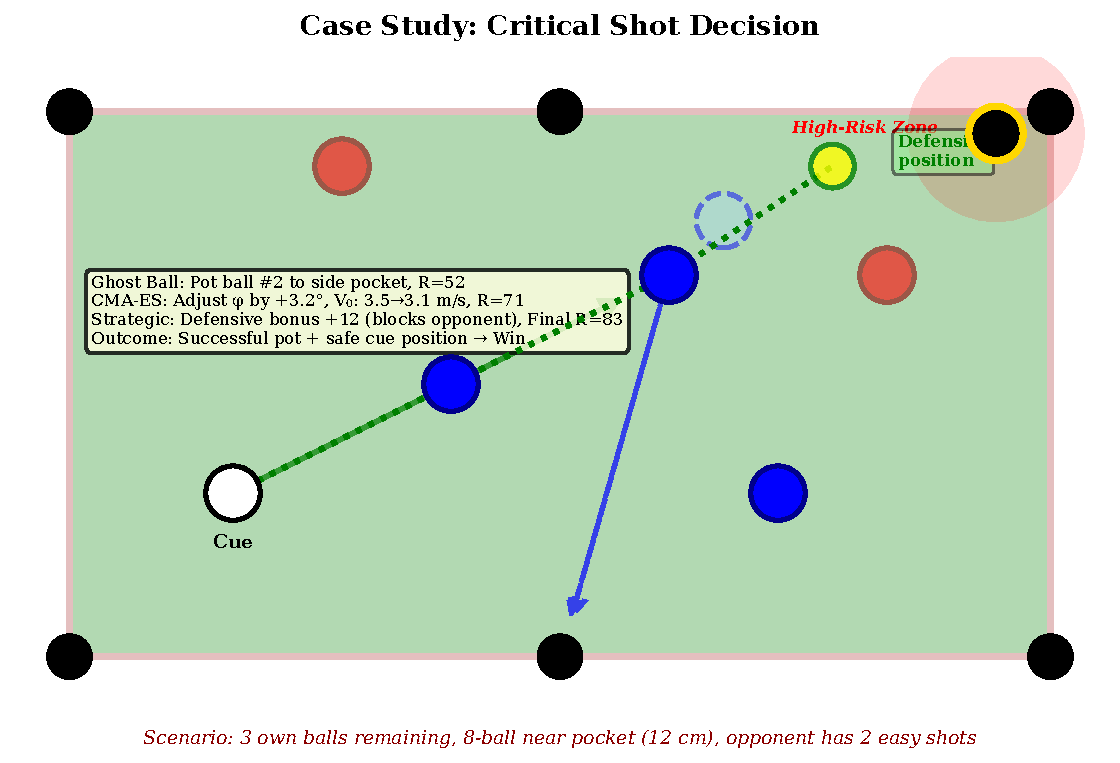
\includegraphics[width=\columnwidth]{figure5_case_study.pdf}
\caption{Case study visualization: a critical state where naive potting may expose catastrophic risk (8-ball near pocket). Ghost Ball provides an initial feasible aim, and selective CMA-ES refines shot parameters to improve robustness under action noise while favoring a safer cue-ball outcome.}
\label{fig:casestudy}
\end{figure}

\textbf{Scenario:} 3 own-group balls remain, opponent has 2 easy shots, 8-ball is 12 cm from corner pocket (high-risk zone).

\textbf{Ghost Ball Output:} Suggests 3-ball pot toward side pocket, $R_{\text{Ghost Ball}} = 52$.

\textbf{CMA-ES Refinement:} Adjusts $\phi$ by $+3.2^\circ$ and $V_0$ from 3.5 to 3.1 m/s, improving pot probability while positioning cue ball behind 8-ball (blocks opponent access to their balls). $R_{\text{CMA-ES}} = 71$.

\textbf{Strategic Evaluation:} Defensive bonus adds $+12$ points due to cue ball placement. Final $R = 83$.

\textbf{Outcome:} Shot successfully pots 3-ball, cue ball ends in safe position. Opponent's next shot requires difficult bank, misses. Agent continues and wins game.

\textbf{Lesson:} The synergy between geometric initialization, local optimization, and strategic evaluation enables robust decision-making in high-pressure scenarios.

\section{CONCLUSION}

This paper presented a hybrid geometric-evolutionary approach to time-constrained 8-ball pool AI, demonstrating that domain-specific structural knowledge can dramatically accelerate black-box optimization without sacrificing decision quality. Through iterative engineering toward a within-time-budget architecture, we illustrated the trade-offs inherent in real-time intelligent systems.

Our key contributions include: (1) intelligent Ghost Ball pruning reducing candidates by $>$50$\times$ (from $\sim$450 to 8), (2) selective CMA-ES refinement applied only when necessary, (3) catastrophic-risk control targeting instant-loss fouls, and (4) strategic bonuses encoding positional and defensive reasoning. Under the course evaluation protocol, the final agent achieves \FinalWinVsBasic\ win rate against BasicAgent and \FinalWinVsPro\ against BasicAgentPro (Table~\ref{table_winrate}).

Ablation studies confirmed that each component contributes meaningfully, with synergistic effects when combined. Particularly, geometric pruning proves to be the critical enabler, allowing expensive evolution strategies to be applied selectively rather than exhaustively.

\subsection{Limitations}

Despite strong performance, several limitations remain:

\textbf{Break Shot Handling:} Our agent treats break shots (opening shot scattering the racked balls) identically to mid-game shots, missing opportunities for specialized break strategies that could improve ball group assignment.

\textbf{Multi-Step Planning:} Current decisions optimize single shots without explicit planning for subsequent shots. While strategic bonuses provide indirect multi-step reasoning through positional rewards, a lookahead search (e.g., 2--3 shots) could improve end-game play.

\textbf{Opponent Modeling:} The agent does not adapt to opponent behavior (e.g., exploiting predictable tendencies). Online opponent modeling could yield marginal win rate gains in extended matches.

\textbf{Offline Training:} We operate in a zero-shot manner without offline learning. Pre-training a value function or policy network could replace hand-crafted reward components with learned representations, potentially improving generalization.

\subsection{Future Directions}

Several promising extensions warrant exploration:

\textbf{Hybrid Neural-Geometric Approaches:} Combine learned value networks (estimating game-theoretic value of resulting states) with geometric shot generation. This could improve defensive play and long-term planning while retaining computational efficiency.

\textbf{Meta-Learning for Adaptive Pruning:} Learn pruning heuristics from historical games to dynamically adjust candidate generation based on table configuration. For instance, increase candidates in complex cluttered states, decrease in simple sparse states.

\textbf{Parallelized Physics Simulation:} Exploit GPU acceleration or distributed computing to evaluate candidates in parallel, potentially allowing more thorough CMA-ES optimization without exceeding time budgets.

\textbf{Transfer to Real-World Robotics:} Adapt the framework to physical billiards robots, addressing additional challenges like visual perception, mechanical actuation noise, and real-time control loop delays.

\textbf{Generalization to Other Domains:} The geometric pruning + selective evolution strategy may transfer to other continuous control domains with structured constraints (e.g., robotic manipulation, drone navigation, industrial process control).

In summary, this work demonstrates that intelligent integration of domain knowledge with general-purpose optimization can yield favorable trade-offs in time-constrained decision-making. The lessons learned—prioritize candidate quality over quantity, adapt computational budget to difficulty, and filter catastrophic failures early—apply broadly to AI systems operating under resource constraints.

\addtolength{\textheight}{-12cm}   % Balance column lengths on last page



%%%%%%%%%%%%%%%%%%%%%%%%%%%%%%%%%%%%%%%%%%%%%%%%%%%%%%%%%%%%%%%%%%%%%%%%%%%%%%%%

\section*{PROJECT CONTRIBUTION AND DIVISION OF LABOR}

\textbf{Team Statement:} This project was completed by a two-person team (Jifan Lin and Yifan Yang). The manuscript is submitted as an individual course report, with the division of labor and contributions summarized below.

\textbf{Jifan Lin (523030910057):}
\begin{itemize}
    \item \textit{Algorithm design and implementation:} Designed and implemented the hybrid Ghost Ball $+$ CMA-ES decision pipeline, including geometric pruning, layered stochastic evaluation, catastrophic foul filtering, and safety/positional shot planning.
    \item \textit{Engineering optimization:} Iteratively profiled runtime bottlenecks and redesigned the pipeline to satisfy time constraints while maintaining competitive win rate.
    \item \textit{Manuscript preparation:} Wrote and typeset this IEEE-format report, including formalization, pseudocode, and experimental discussion.
\end{itemize}

\textbf{Yifan Yang (523030910054):}
\begin{itemize}
    \item \textit{Evaluation infrastructure and reproducibility:} Prepared and maintained the evaluation environment, validated baseline agents, and ensured tournament-style testing is reproducible across machines and seeds.
    \item \textit{Ablation study leadership:} Led the design and execution of ablation experiments (Table~\ref{table_ablation}), including selecting ablation variants, running large-$N$ match suites, and cross-checking summaries/plots for consistency.
    \item \textit{Hyperparameter tuning and robustness:} Performed targeted tuning and stress testing (candidate caps, sampling schedules, pruning thresholds, and strategy weights), contributing to improved win rate and runtime stability under stochastic action noise.
    \item \textit{Review and quality control:} Systematically reviewed results, figures, and manuscript consistency (numbers, units, and captions), and provided feedback that improved clarity and compliance with course requirements.
\end{itemize}



%%%%%%%%%%%%%%%%%%%%%%%%%%%%%%%%%%%%%%%%%%%%%%%%%%%%%%%%%%%%%%%%%%%%%%%%%%%%%%%%

\section*{ACKNOWLEDGMENT}

The authors thank the AI3603 course staff at Shanghai Jiao Tong University for providing the Pooltool simulation environment and baseline agents. Special thanks to the developers of the Pooltool library for maintaining an open-source, high-fidelity billiards physics engine. This project was completed collaboratively by a two-person team; this manuscript is submitted as an individual course report with the division of labor stated above.



%%%%%%%%%%%%%%%%%%%%%%%%%%%%%%%%%%%%%%%%%%%%%%%%%%%%%%%%%%%%%%%%%%%%%%%%%%%%%%%%

\bibliographystyle{IEEEtran}
\bibliography{references}




\end{document}
